\documentclass{mrl}

\title{Dynamic block size algorithms with an exponential upper bound on growth are vulnerable to bloat attack vectors}
\authors{Isthmus\footnote{\texttt{Isthmus@getmonero.org} ** PENDING SETUP **}}
\affiliations{Monero Research Lab, Noncesense Research Lab}
\date{December 2018}

\usepackage[official]{eurosym}

\usepackage{draftwatermark}
\SetWatermarkScale{4}
\SetWatermarkLightness{0.9}

\type{TECHNICAL NOTE}
\ident{MRL-0012}

\begin{document}
\vspace{-0.25cm}
\begin{abstract}
This note quantifies the maximum damage (in terms of block size and blockchain size) that any spam-based attack vector could cause in protocols that employ a dynamic block size algorithm without appropriate upper bounds on continuous growth. Under non-adversarial conditions, excessive growth is discouraged by a miner reward penalty for creating oversize blocks, however an attacker can override the normal cryptoeconomic safeguards by creating sets of transactions whose net fee is greater than the coinbase reward, and whose net weight matches the maximum allowed block size. The numeric simulations presented here demonstrate that an adversary could disable most or all Monero nodes within a day, which could only be retroactively repaired by a soft fork to censor transactions that were previously included in the blockchain.
\end{abstract}

\section{Introduction}
The current bound on expansion of the Monero blockchain is that each block cannot be larger than the median size of the previous 100 blocks. Given the 2-minute average block time, this means that the protocol has a 3.3-hour memory, which performs well under normal use patterns. However, it is prudent to consider edge cases as well - the current absence of medium or long-term memory leaves the network susceptible to catastrophic block size inflation. 

\section{Threat model}
A well-funded adversary wishes to disrupt the Monero cryptocurrency/network/community, so they create a set of transactions whose net weight is equal to the maximum allowed block size, and whose net fees are greater than the coinbase. Given all of the possible subsets of transactions in the memory pool (and taking into account the coinbase penalty), the attacker's transactions must be the most profitable permutation. This induces miners to create a maximum-size block, filled with the attacker's spam at the expense of legitimate transactions.

By repeating this process with every sequential block, the attacker continually increases the block size at the maximum rate allowed by the consensus protocol.  The attacker only needs to pay penalty-overriding fees to \emph{increase} the block size; maintaining the large blocks is inexpensive under the current algorithm. Thus an attacker could pay a premium to escalate the block size to 1 GB, and sustain that block size indefinitely with minimal ongoing costs. Note: the attacker does not mine; they only create sets of transactions that honest miners are incentivized to select. 

\section{Simulation methods}
Numeric simulations were carried out to study blockchain growth under three different approaches to block size limit:
\begin{itemize}
    \item \textbf{Current limit:} Each block is limited to twice the median size of the previous 100 blocks. Since block size increase is multiplicative, blockchain growth (its integral) is exponential.
    \item \textbf{Additive limit:} Each block is allowed to grow by a fixed increment, e.g. +300 kB. With an additive block size increase, blockchain growth is linear with respect to time and cost.
    \item\textbf{Dynamic algorithm with fixed cap:} A \textit{temporary} fixed block size cap could be prepared to harden Monero against this attack (without otherwise modifying the current dynamic block size algorithm). This could be added as an emergency fail-safe to prevent exploitation while a long-term solution is discussed.
\end{itemize}
This is \textbf{not} an exhaustive list of mitigation strategies, and readers are encouraged to model and/or submit their own ideas. Other methods were proposed during the public 2018-11-26 Monero Research Lab, such as block size momentum, nonlinear penalties, and hashrate-informed growth limits. Alternately, the \emph{accumulated} growth could be bounded by allocating a maximum blockchain size increase between upgrade forks (e.g. 1 TB max between Oct 2019 and March 2020), implementing a secondary fail-safe limit based on the number of blocks until the next upgrade, and the remaining space budget.

Simulations use a 3.5 XMR block reward, and the 35 \EUR{}/XMR exchange rate at time of writing. Note that overriding the penalty results in suppression of all coin emission, so the block reward remains fixed throughout the attack. The exchange rate would likely skew against Monero as the attack proceeds and users attempt to convert their funds before the network is disabled.

\section{Observations}
Results of the simulation are described textually in table \ref{results_table}. The current method results in gigabyte-scale blocks within 24 hours, while the overall blockchain becomes tens of terabytes in less than 36 hours. Figures \ref{fig_block_size} and \ref{fig_chain_size} show the increase in block size and blockchain size over the course of a 36-hour attack. Figure \ref{fig_bloat_rate} shows the amount of damage as a function of fiat cost to the attacker.

Numeric simulations demonstrate that an adversary could theoretically drive the blockchain to 30 TB within 36 hours, however most nodes will probably be disabled within the first day due to insufficient bandwidth and computational resources to distribute and validate 3 GB blocks. This one-time attack to permanently disable the Monero network or force a controversial soft-fork rollback costs approximately 90,000\EUR{} at the time of writing.
 
The attacker only needs to pay penalty-overriding fees to \emph{increase} the block size; maintaining the large blocks is inexpensive under the current algorithm. Thus an attacker could pay a premium to escalate the block size to 1 GB, and sustain that block size indefinitely with minimal ongoing costs.
 
Most cryptoeconomic schemes include fee/reward mechanisms designed to discourage undesired behavior from financially-rational parties (i.e. the vast majority of users, whose aim to preserve/increase their position in that cryptocurrrency). However all protocols \textit{must} include secondary fail-safe mechanisms to protect the networks against adversaries whose external agendas override economic motivations.


\begin{table}
\centering 
\begin{tabular}{l | c c c c c} %
\hline
\hline
\textbf{Hours into attack:} & \textbf{6h} & \textbf{12h} & \textbf{18h} & \textbf{24h} & \textbf{36h}\\
Total cost to attacker (\EUR{}) & 22,000 & 44,000 & 66,000 & 88,000 & 132,000\\
Total cost to attacker (XMR) & 630 & 1260 & 1890 & 2520 & 3780 \\
Stake of total supply needed & 0.004\% & 0.008 \% & 0.012 \% & 0.016 \% & 0.018 \% \\
\hline
& \multicolumn{5}{c}{\textbf{Block size (MB)}} \\ 
Current method (x2 per 100 blocks) & 1.6 & 25 & 200 & 3300 & 420000\\
Additive (+300 kB per block) & 1.3 & 2.5 & 3.4 & 4.6 & 6.7 \\
Temporary stop-gap (5 MB hard cap) & 1.6 & 5 & 5 & 5 & 5 \\
& \multicolumn{5}{c}{\textbf{Blockchain size (GB)}} \\ 
Current method (x2 per 100 blocks) & 65 & 66 & 82 & 270 & 30000\\
Additive (+300 kB per block) & 65 & 65 & 66 & 67 & 69 \\
Temporary stop-gap (5 MB hard cap) & 65 & 66 & 67 & 68 & 69 \\
\hline\hline
\end{tabular}
\caption{Performance of various dynamic block size limit algorithms during a simulated 36-hour attack} 
\label{results_table}
\end{table}

\begin{figure}[p]
    \centering
    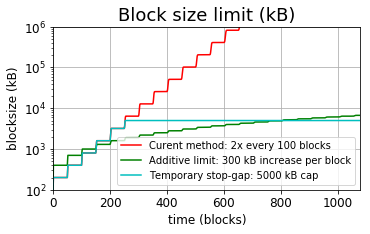
\includegraphics[scale=0.7]{fig_block_size.png}
    \caption{Block size over a 36-hour attack simulation}
    \label{fig_block_size}
\end{figure}

\begin{figure}[p]
    \centering
    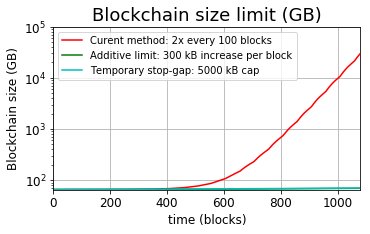
\includegraphics[scale=0.7]{fig_chain_size.png}
    \caption{Blockchain size over a 36-hour attack simulation}
    \label{fig_chain_size}
\end{figure}

\begin{figure}[p]
    \centering
    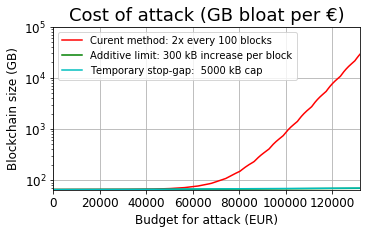
\includegraphics[scale=0.7]{fig_bloat_rate.png}
    \caption{Cost of the attack at time of writing}
    \label{fig_bloat_rate}
\end{figure}

\end{document}